% Editable native annotations around unchanged verified IDE photographs.
\par
\begin{figure}[htbp]
\centering
\newsavebox{\MARSmatmulsegmentregistersBox}
\sbox{\MARSmatmulsegmentregistersBox}{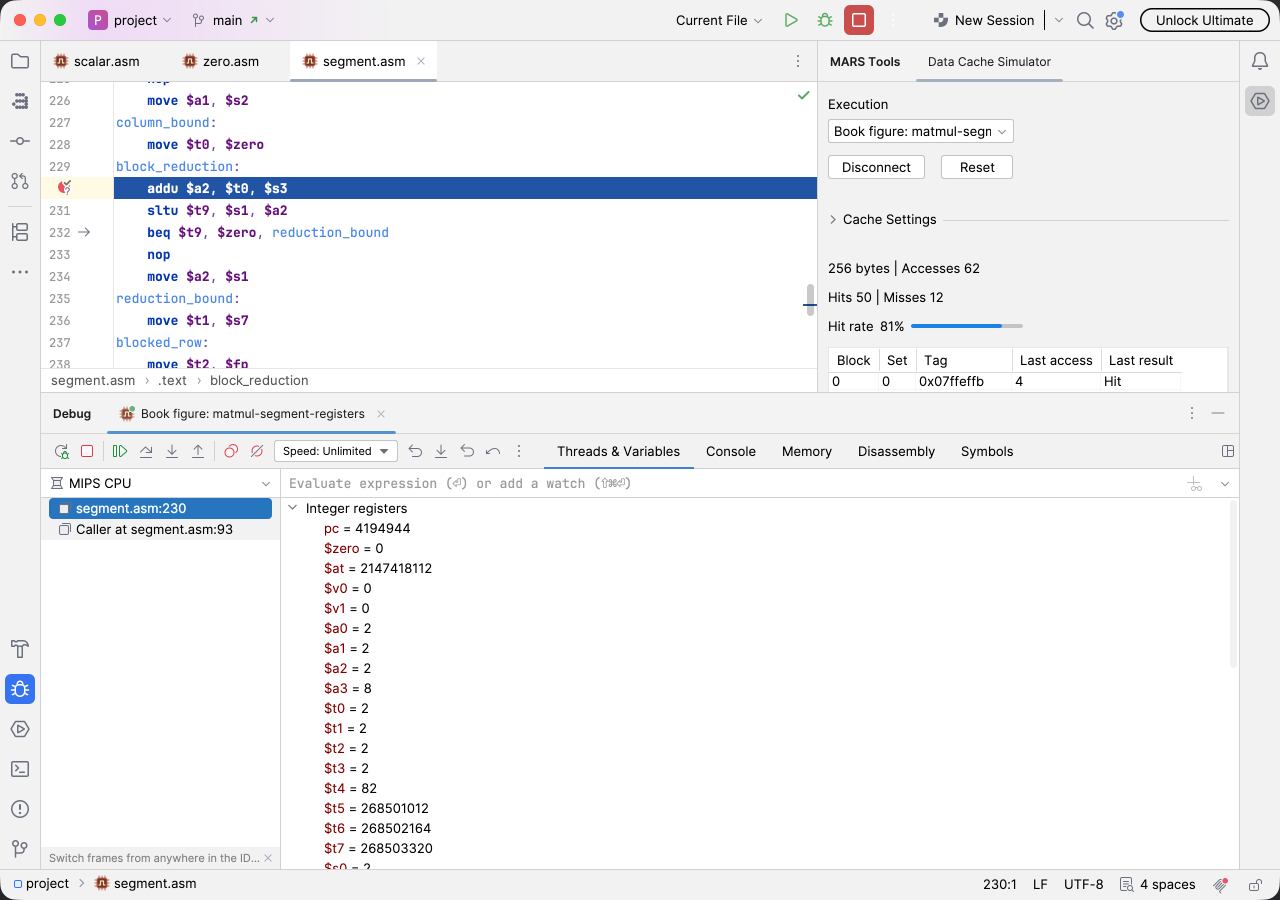
\includegraphics[artifact]{packages/022-blocked-matmul/captures/f03/registers.png}}
\newsavebox{\MARSmatmulsegmentproductBox}
\sbox{\MARSmatmulsegmentproductBox}{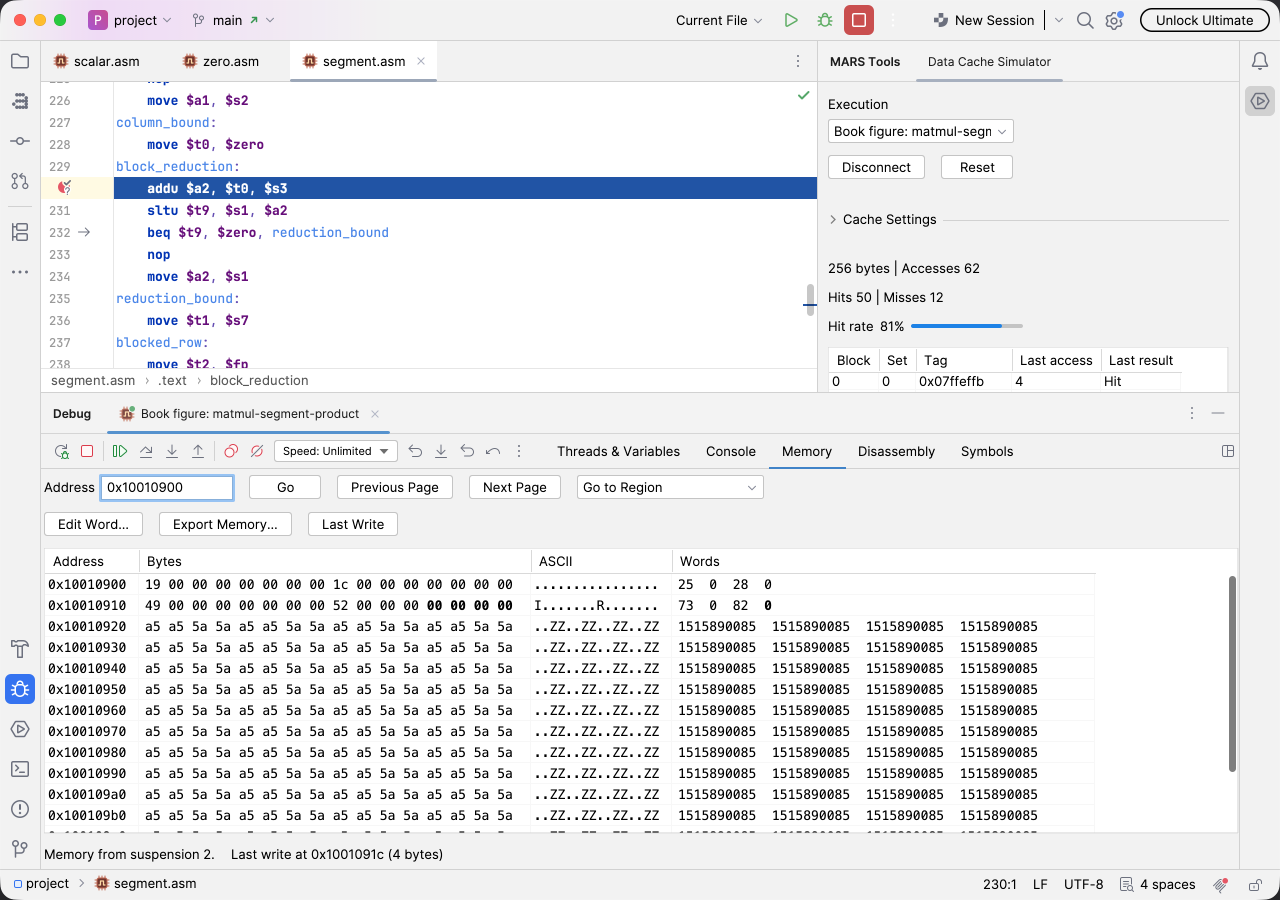
\includegraphics[artifact]{packages/022-blocked-matmul/captures/f03/product.png}}
\newsavebox{\MARSmatmulsegmentcallerBox}
\sbox{\MARSmatmulsegmentcallerBox}{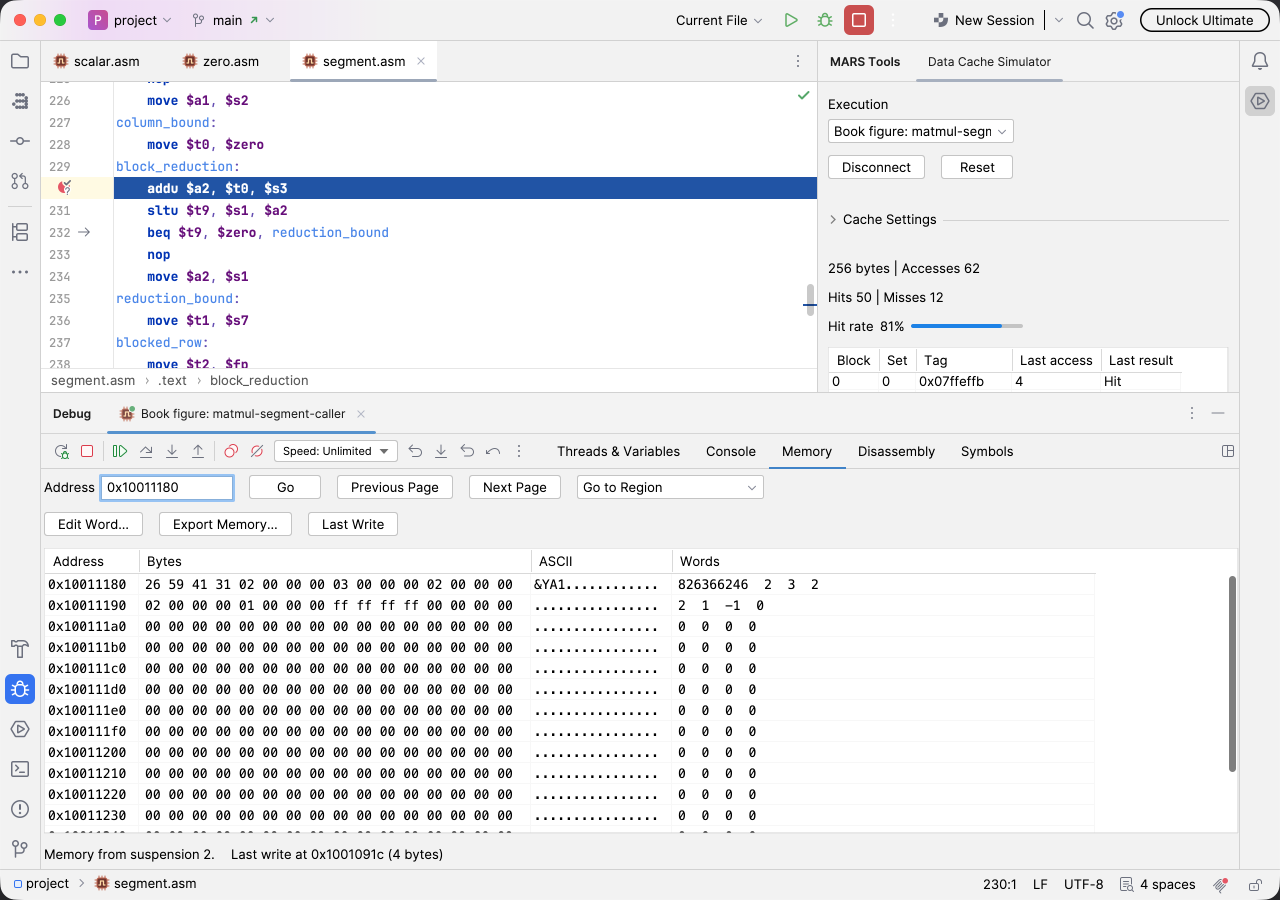
\includegraphics[artifact]{packages/022-blocked-matmul/captures/f03/caller.png}}
\edef\MARSmatmulsegmentsourceLeft{\the\dimexpr0.036718750\wd\MARSmatmulsegmentregistersBox\relax}
\edef\MARSmatmulsegmentsourceBottom{\the\dimexpr0.774444444\ht\MARSmatmulsegmentregistersBox\relax}
\edef\MARSmatmulsegmentsourceRight{\the\dimexpr0.713281250\wd\MARSmatmulsegmentregistersBox\relax}
\edef\MARSmatmulsegmentsourceTop{\the\dimexpr0.170000000\ht\MARSmatmulsegmentregistersBox\relax}
\edef\MARSmatmulsegmentregistersLeft{\the\dimexpr0.246093750\wd\MARSmatmulsegmentregistersBox\relax}
\edef\MARSmatmulsegmentregistersBottom{\the\dimexpr0.201111111\ht\MARSmatmulsegmentregistersBox\relax}
\edef\MARSmatmulsegmentregistersRight{\the\dimexpr0.553906250\wd\MARSmatmulsegmentregistersBox\relax}
\edef\MARSmatmulsegmentregistersTop{\the\dimexpr0.773333333\ht\MARSmatmulsegmentregistersBox\relax}
\edef\MARSmatmulsegmentproductLeft{\the\dimexpr0.034375000\wd\MARSmatmulsegmentproductBox\relax}
\edef\MARSmatmulsegmentproductBottom{\the\dimexpr0.311111111\ht\MARSmatmulsegmentproductBox\relax}
\edef\MARSmatmulsegmentproductRight{\the\dimexpr0.584375000\wd\MARSmatmulsegmentproductBox\relax}
\edef\MARSmatmulsegmentproductTop{\the\dimexpr0.608888889\ht\MARSmatmulsegmentproductBox\relax}
\edef\MARSmatmulsegmentcallerLeft{\the\dimexpr0.034375000\wd\MARSmatmulsegmentcallerBox\relax}
\edef\MARSmatmulsegmentcallerBottom{\the\dimexpr0.311111111\ht\MARSmatmulsegmentcallerBox\relax}
\edef\MARSmatmulsegmentcallerRight{\the\dimexpr0.584375000\wd\MARSmatmulsegmentcallerBox\relax}
\edef\MARSmatmulsegmentcallerTop{\the\dimexpr0.608888889\ht\MARSmatmulsegmentcallerBox\relax}
\begin{tikzpicture}[alt={Four annotated details at the second block_reduction visit show t0 equal two, partial output doublewords 25 28 73 82, shape two three two two and completed minus one. The next segment adds the final reduction position to produce 58 64 139 154.}]
\node[anchor=north west,inner sep=0,font=\small\bfseries] (source-title) at (6mm,0) {Next instruction at this boundary};
\node[anchor=north west,inner sep=0] (source) at ([yshift=-1mm]source-title.south west) {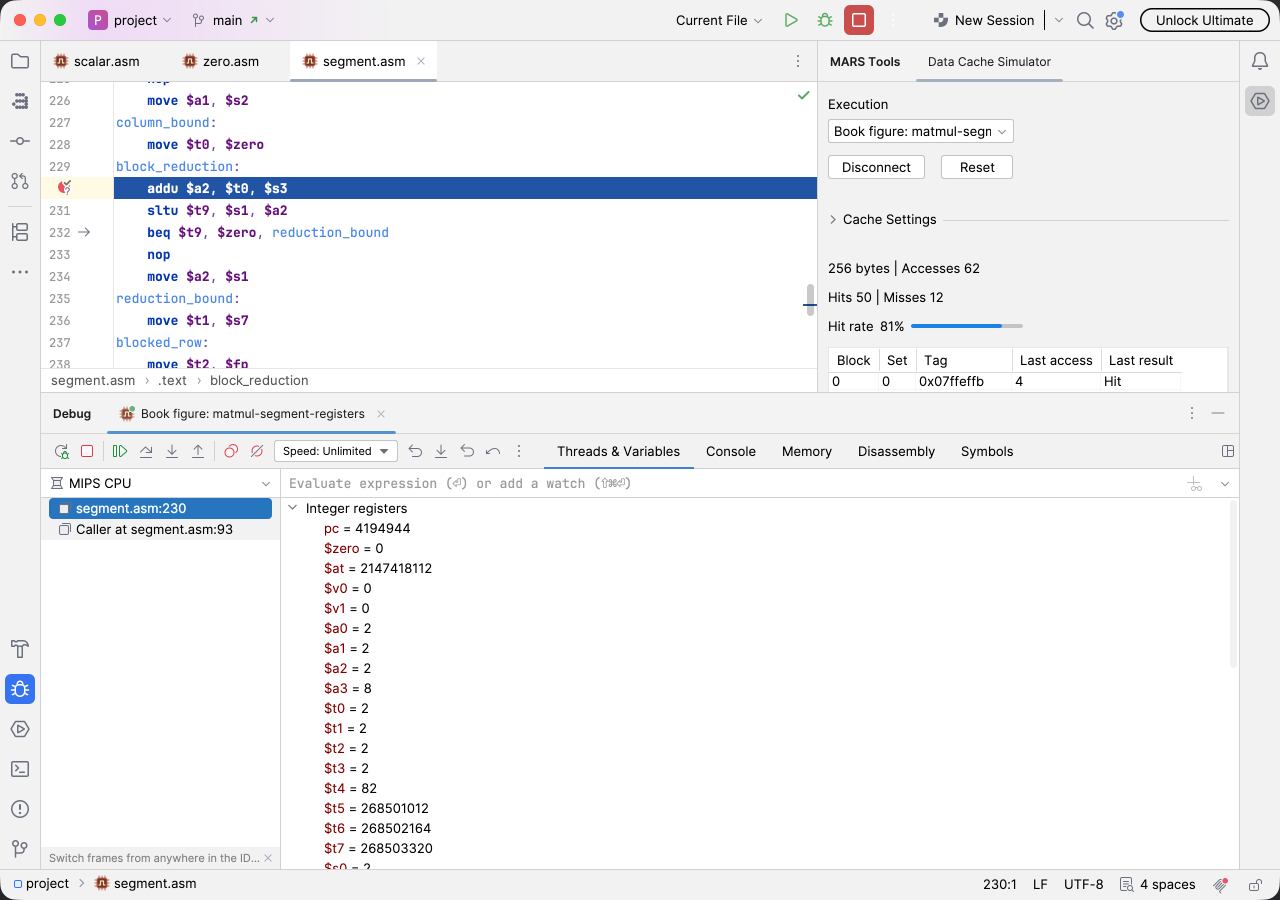
\includegraphics[width=0.54\linewidth,artifact,trim={\MARSmatmulsegmentsourceLeft{} \MARSmatmulsegmentsourceBottom{} \MARSmatmulsegmentsourceRight{} \MARSmatmulsegmentsourceTop{}},clip]{packages/022-blocked-matmul/captures/f03/registers.png}};
\begin{scope}[shift={(source.south west)},x={($(source.south east)-(source.south west)$)},y={($(source.north west)-(source.south west)$)}]
\draw[black,line width=0.7pt] (0.215625000,0.080000000) rectangle (0.750000000,0.520000000);
\node[draw=black,fill=white,circle,inner sep=1.5pt,font=\footnotesize] at ($(0.215625000,0.520000000)+(-3mm,0)$) {1};
\end{scope}
\node[anchor=north west,inner sep=0,font=\small\bfseries] (registers-title) at (0.58\linewidth,0 |- source-title.north) {Register value at this boundary};
\node[anchor=north west,inner sep=0] (registers) at ([yshift=-1mm]registers-title.south west) {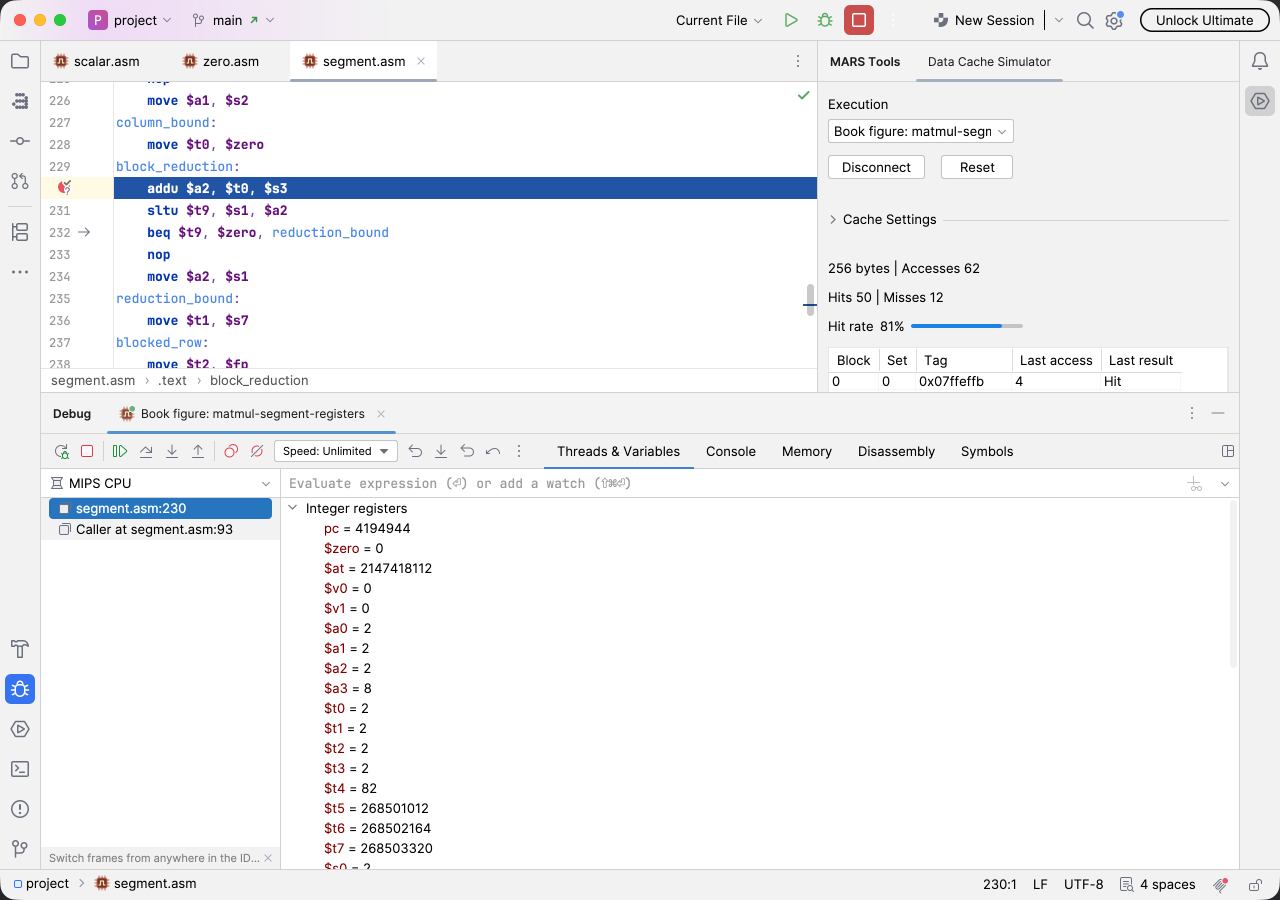
\includegraphics[width=0.42\linewidth,artifact,trim={\MARSmatmulsegmentregistersLeft{} \MARSmatmulsegmentregistersBottom{} \MARSmatmulsegmentregistersRight{} \MARSmatmulsegmentregistersTop{}},clip]{packages/022-blocked-matmul/captures/f03/registers.png}};
\begin{scope}[shift={(registers.south west)},x={($(registers.south east)-(registers.south west)$)},y={($(registers.north west)-(registers.south west)$)}]
\draw[black,line width=0.7pt] (0.023437500,0.043478261) rectangle (0.214843750,0.913043478);
\node[draw=black,fill=white,circle,inner sep=1.5pt,font=\footnotesize] at ($(0.023437500,0.913043478)+(-3mm,0)$) {2};
\end{scope}
\node[anchor=north west,inner sep=0,font=\small\bfseries] (product-title) at ([yshift=-1mm]source.south west) {Output doublewords};
\node[anchor=north west,inner sep=0] (product) at ([yshift=-1mm]product-title.south west) {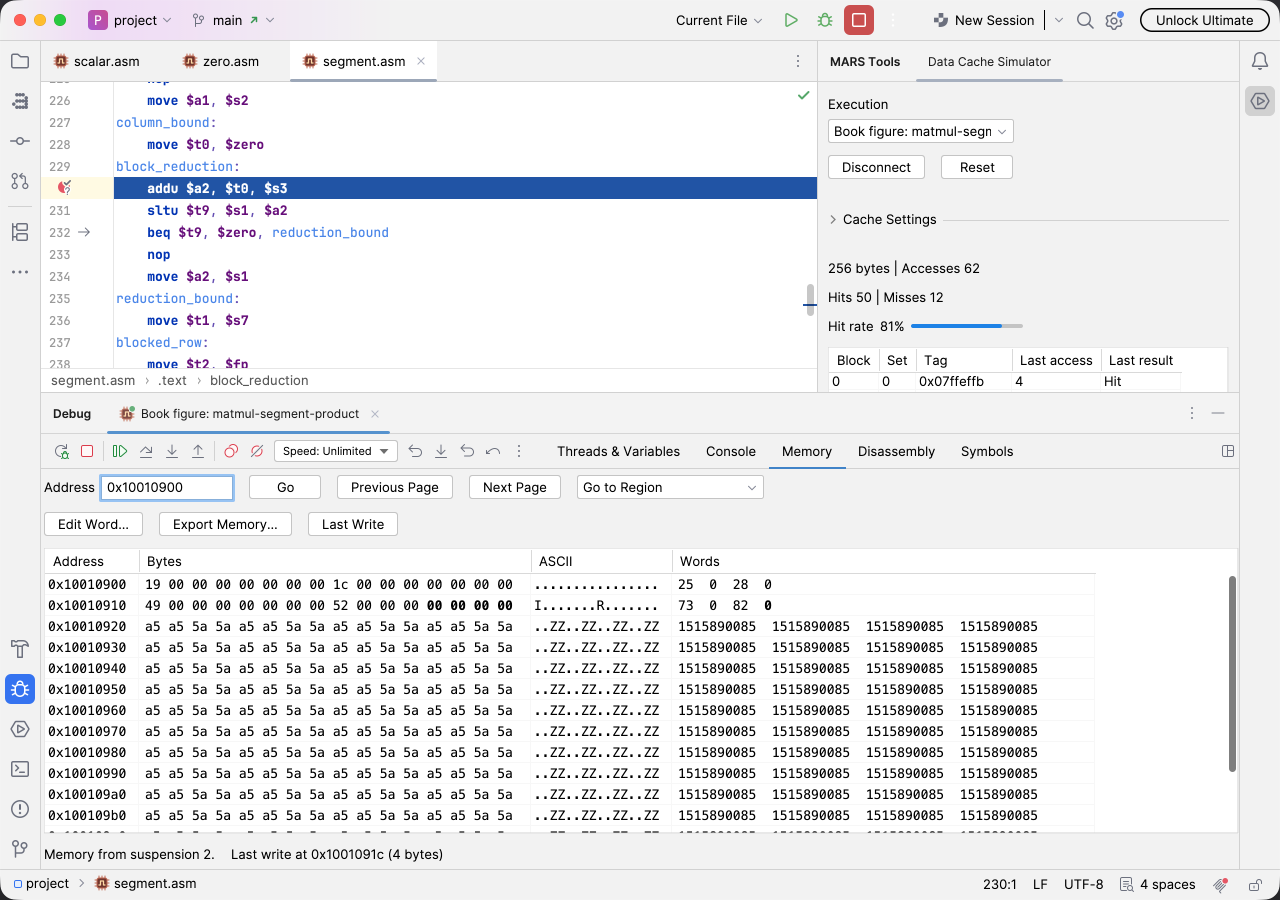
\includegraphics[width=0.84\linewidth,artifact,trim={\MARSmatmulsegmentproductLeft{} \MARSmatmulsegmentproductBottom{} \MARSmatmulsegmentproductRight{} \MARSmatmulsegmentproductTop{}},clip]{packages/022-blocked-matmul/captures/f03/product.png}};
\begin{scope}[shift={(product.south west)},x={($(product.south east)-(product.south west)$)},y={($(product.north west)-(product.south west)$)}]
\draw[black,line width=0.7pt] (0.194672131,0.055555556) rectangle (0.997950820,0.638888889);
\node[draw=black,fill=white,circle,inner sep=1.5pt,font=\footnotesize] at ($(0,0.638888889)+(-3mm,0)$) {3};
\end{scope}
\node[anchor=north west,inner sep=0,font=\small\bfseries] (caller-title) at ([yshift=-1mm]product.south west) {Shape, method and saved count};
\node[anchor=north west,inner sep=0] (caller) at ([yshift=-1mm]caller-title.south west) {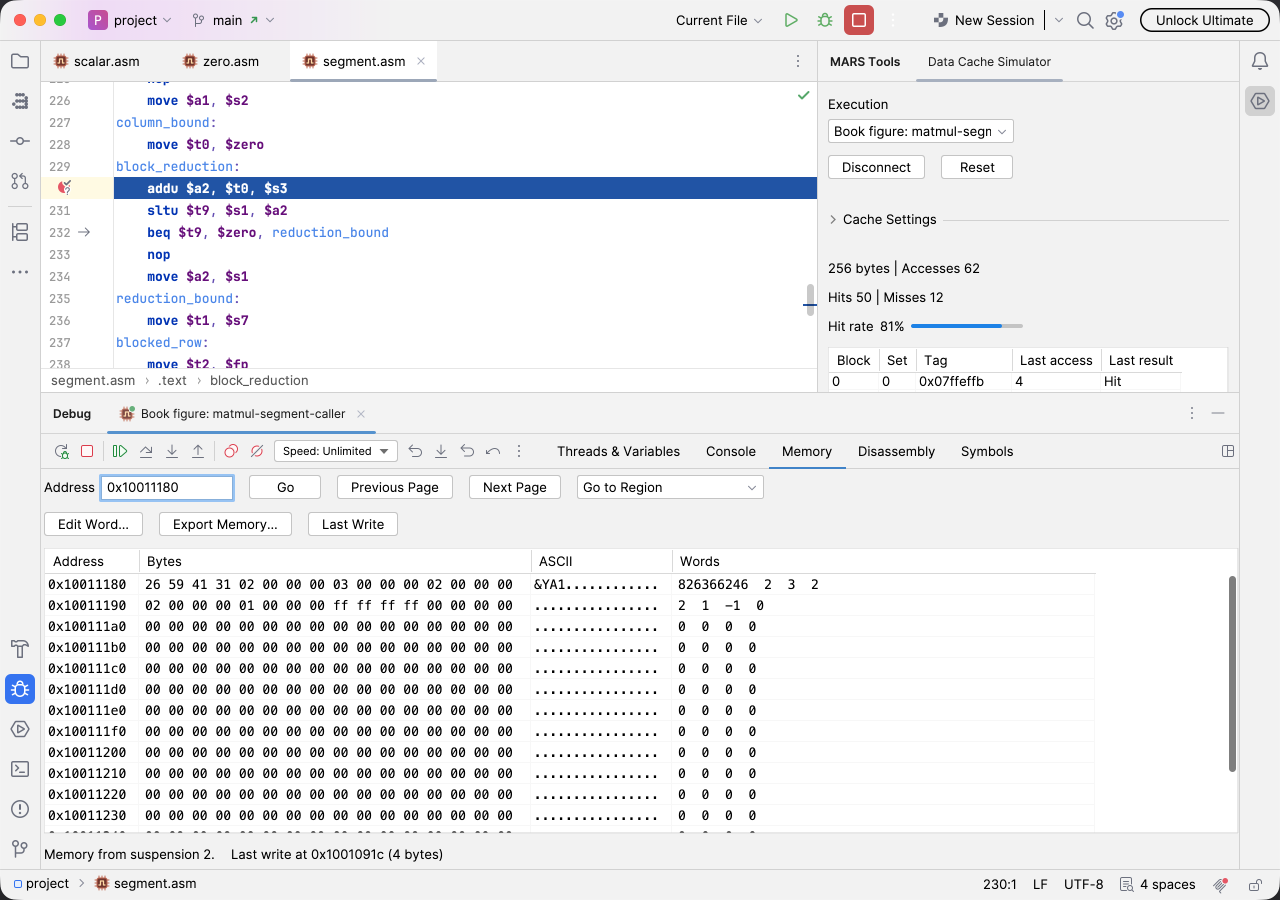
\includegraphics[width=0.84\linewidth,artifact,trim={\MARSmatmulsegmentcallerLeft{} \MARSmatmulsegmentcallerBottom{} \MARSmatmulsegmentcallerRight{} \MARSmatmulsegmentcallerTop{}},clip]{packages/022-blocked-matmul/captures/f03/caller.png}};
\begin{scope}[shift={(caller.south west)},x={($(caller.south east)-(caller.south west)$)},y={($(caller.north west)-(caller.south west)$)}]
\draw[black,line width=0.7pt] (0.194672131,0.055555556) rectangle (0.997950820,0.638888889);
\node[draw=black,fill=white,circle,inner sep=1.5pt,font=\footnotesize] at ($(0,0.638888889)+(-3mm,0)$) {4};
\end{scope}
\end{tikzpicture}
\par\smallskip
\begin{minipage}{\linewidth}
\small
\begin{enumerate}
\setlength{\itemsep}{2pt}
\setlength{\parsep}{0pt}
\item The conditional breakpoint stops at the second \texttt{block\_reduction} visit, before computing its clipped end. One reduction segment has completed; the function has not returned.
\item \texttt{t0 = 2} is the next reduction start $L$. The preceding segment covered $k=0,1$; the remaining segment contains only $k=2$, because $K=3$ and $T=2$.
\item Output retains $(25,28)$ and $(73,82)$. For example, $25=1\cdot7+2\cdot9$. The next segment adds $(33,36)$ and $(66,72)$, producing $(58,64)$ and $(139,154)$. Resetting these partial sums would discard valid work.
\item The shape remains $2,3,2,2$, method is one, and \texttt{completed} remains $-1$. These are partial cell values, not a completed call. No return count is inferred from an internal register state.
\end{enumerate}
\end{minipage}
\caption{The second reduction tile begins with the first segment already retained in output.}
\label{capture:022-blocked-matmul-f03}
\label{matmul-f03}
\end{figure}
\par
